%%% --- Bartholomew2019.tex
%%
%%% Single slide for one minute poster presentation at High-Performance numerical algorithms
%%  meeting.

\documentclass[
9pt,
linkcolor=red,
urlcolor=blue
]{beamer}

\usepackage{epstopdf}

\newcommand{\subrule}{\vspace{0.1cm}\hrule}

\setbeamertemplate{navigation symbols}{}
\setbeamertemplate{footline}[text line]{
  \parbox{\linewidth}{\vspace*{-8pt}Numerical algorithms for high-performance computational science\hfill
    2019\hfill Paul Bartholomew, Georgios Deskos, Sylvain Laizet}
}
\setbeamertemplate{itemize items}[circle]

\begin{document}

\begin{frame}
  \frametitle{Xcompact3d: Modernising and expanding the capabilities of the high-order flow solver
    Incompact3d\subrule}
  \vspace{-20pt}

  \begin{columns}
    \begin{column}{0.5\textwidth}
      \begin{itemize}
      \item Navier-Stokes solver aimed at LES and DNS simulations of turbulent flows
      \item Scalability up to $\mathcal{O} \left( 10^5 \right)$ CPUs achieved through
        \begin{itemize}
        \item 2D domain decomposition
        \item Compact finite difference schemes
        \item Direct spectral Poisson solver
        \end{itemize}
      \item Multiple capabilities including
        \begin{itemize}
        \item Complex domains through IBM
        \item Variable-density low Mach number flows
        \item Wind farm simulation
        \end{itemize}
      \item Open source: \url{github.com/xcompact3d}
      \end{itemize}
    \end{column}
    \begin{column}{0.5\textwidth}
      \begin{figure}[h]
        \centering
        \includegraphics[width=0.9\textwidth]{./pencil_decomp}
        \caption{Domain decomposition}
      \end{figure}
      \vspace{-20pt}
      \begin{figure}[h]
        \centering
        \def\svgwidth{\textwidth}
        %% Creator: Inkscape inkscape 0.91, www.inkscape.org
%% PDF/EPS/PS + LaTeX output extension by Johan Engelen, 2010
%% Accompanies image file '3D_view.eps' (pdf, eps, ps)
%%
%% To include the image in your LaTeX document, write
%%   \input{<filename>.pdf_tex}
%%  instead of
%%   \includegraphics{<filename>.pdf}
%% To scale the image, write
%%   \def\svgwidth{<desired width>}
%%   \input{<filename>.pdf_tex}
%%  instead of
%%   \includegraphics[width=<desired width>]{<filename>.pdf}
%%
%% Images with a different path to the parent latex file can
%% be accessed with the `import' package (which may need to be
%% installed) using
%%   \usepackage{import}
%% in the preamble, and then including the image with
%%   \import{<path to file>}{<filename>.pdf_tex}
%% Alternatively, one can specify
%%   \graphicspath{{<path to file>/}}
%% 
%% For more information, please see info/svg-inkscape on CTAN:
%%   http://tug.ctan.org/tex-archive/info/svg-inkscape
%%
\begingroup%
  \makeatletter%
  \providecommand\color[2][]{%
    \errmessage{(Inkscape) Color is used for the text in Inkscape, but the package 'color.sty' is not loaded}%
    \renewcommand\color[2][]{}%
  }%
  \providecommand\transparent[1]{%
    \errmessage{(Inkscape) Transparency is used (non-zero) for the text in Inkscape, but the package 'transparent.sty' is not loaded}%
    \renewcommand\transparent[1]{}%
  }%
  \providecommand\rotatebox[2]{#2}%
  \ifx\svgwidth\undefined%
    \setlength{\unitlength}{2620.65566406bp}%
    \ifx\svgscale\undefined%
      \relax%
    \else%
      \setlength{\unitlength}{\unitlength * \real{\svgscale}}%
    \fi%
  \else%
    \setlength{\unitlength}{\svgwidth}%
  \fi%
  \global\let\svgwidth\undefined%
  \global\let\svgscale\undefined%
  \makeatother%
  \begin{picture}(1,0.64218702)%
    \put(0,0){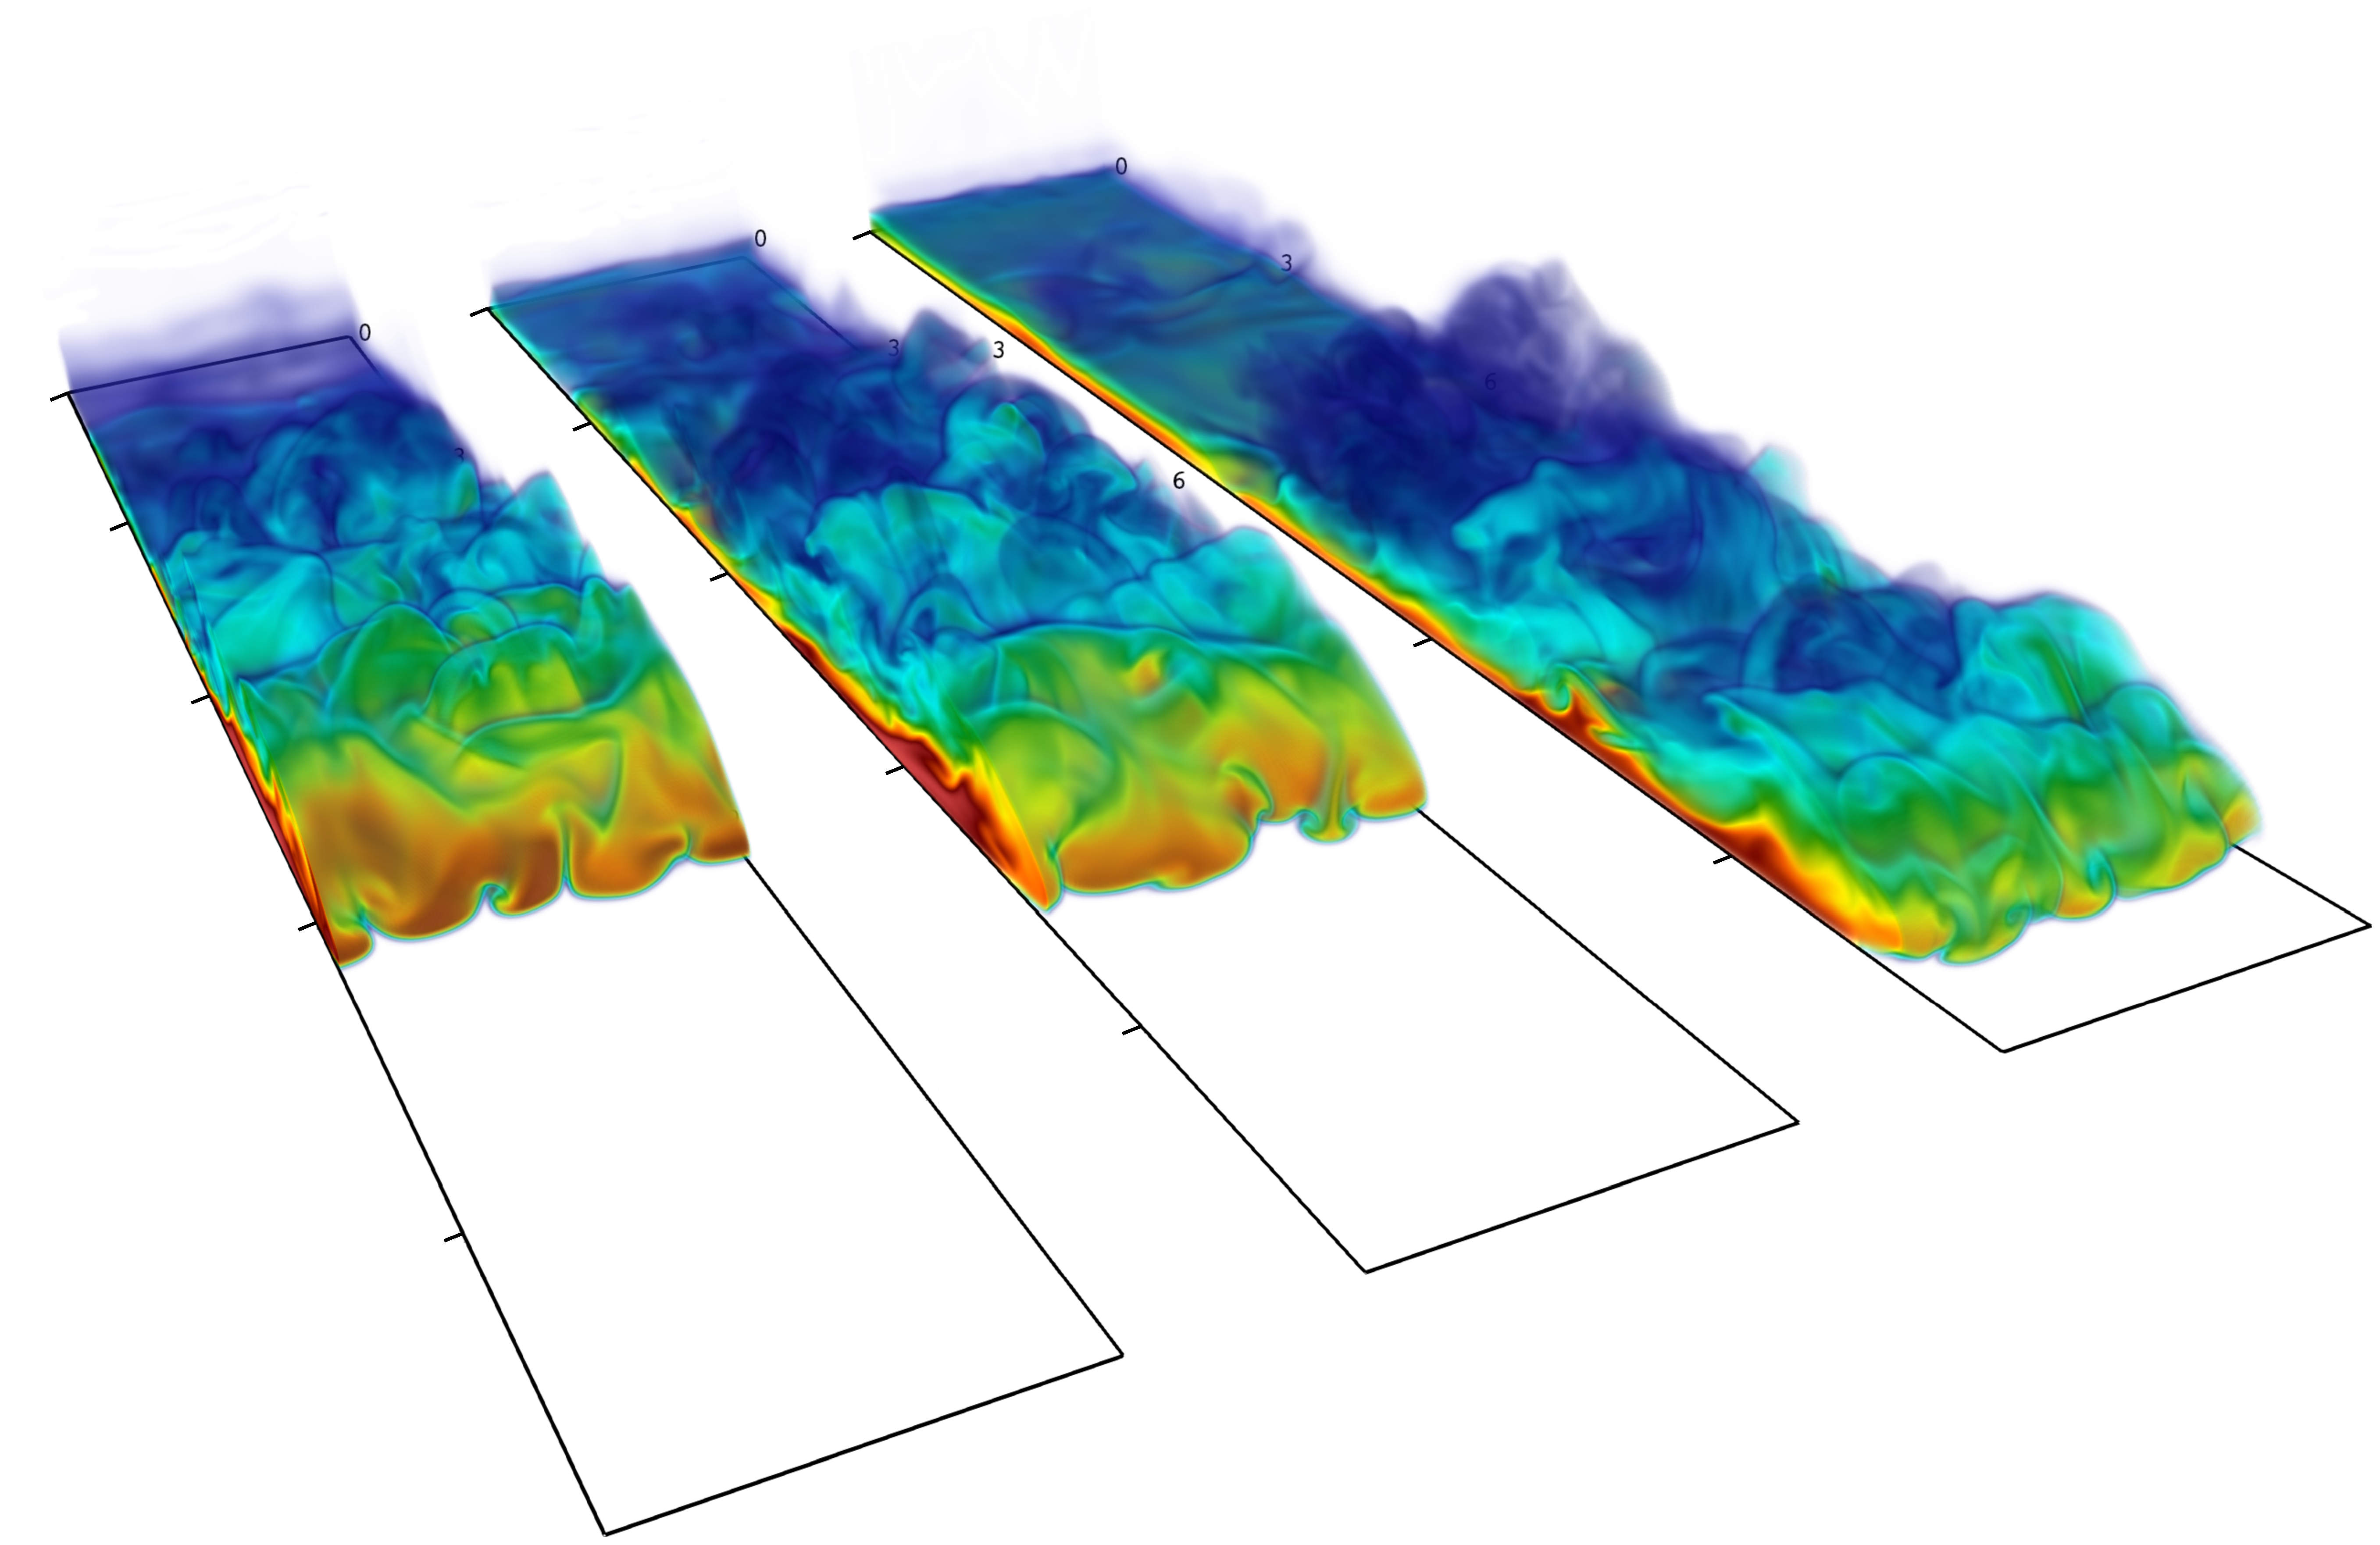
\includegraphics[width=\unitlength]{./3D_view.eps}}%
    \put(0.00145919,0.46921291){\color[rgb]{0,0,0}\makebox(0,0)[lb]{\smash{$0$}}}%
    \put(0.02837803,0.41458666){\color[rgb]{0,0,0}\makebox(0,0)[lb]{\smash{$3$}}}%
    \put(0.06243918,0.34223246){\color[rgb]{0,0,0}\makebox(0,0)[lb]{\smash{$6$}}}%
    \put(0.1070291,0.2479021){\color[rgb]{0,0,0}\makebox(0,0)[lb]{\smash{$9$}}}%
    \put(0.15773926,0.11672119){\color[rgb]{0,0,0}\makebox(0,0)[lb]{\smash{$12$}}}%
    \put(0.18060364,0.50402948){\color[rgb]{0,0,0}\makebox(0,0)[lb]{\smash{$0$}}}%
    \put(0.33972687,0.53683966){\color[rgb]{0,0,0}\makebox(0,0)[lb]{\smash{$0$}}}%
    \put(0.22326914,0.45643631){\color[rgb]{0,0,0}\makebox(0,0)[lb]{\smash{$3$}}}%
    \put(0.28050814,0.39309198){\color[rgb]{0,0,0}\makebox(0,0)[lb]{\smash{$6$}}}%
    \put(0.35364644,0.31285474){\color[rgb]{0,0,0}\makebox(0,0)[lb]{\smash{$9$}}}%
    \put(0.57496175,0.36634375){\color[rgb]{0,0,0}\makebox(0,0)[lb]{\smash{$9$}}}%
    \put(0.44430417,0.20442073){\color[rgb]{0,0,0}\makebox(0,0)[lb]{\smash{$12$}}}%
    \put(0.69146617,0.27592795){\color[rgb]{0,0,0}\makebox(0,0)[lb]{\smash{$12$}}}%
  \end{picture}%
\endgroup%

        \caption{Gravity currents at different density ratios}
      \end{figure}
    \end{column}
  \end{columns}
  
\end{frame}

\end{document}


%%% Local Variables:
%%% mode: latex
%%% TeX-master: t
%%% End:
